%%%%%%%%%%%%%%%%%%%%%%%%%%%%%%%%%%%%%%%%%%%%%%%%%%%%%%%%%%%%%%%%%%
%%%%%%%% ICML 2016 EXAMPLE LATEX SUBMISSION FILE %%%%%%%%%%%%%%%%%
%%%%%%%%%%%%%%%%%%%%%%%%%%%%%%%%%%%%%%%%%%%%%%%%%%%%%%%%%%%%%%%%%%

% Use the following line _only_ if you're still using LaTeX 2.09.
%\documentstyle[icml2016,epsf,natbib]{article}
% If you rely on Latex2e packages, like most moden people use this:
\documentclass[accepted]{article} % With author names, without line numbers
% \documentclass{article} % without author names, with line numbers

% use Times
\usepackage{times}
% For figures
\usepackage{graphicx} % more modern
%\usepackage{epsfig} % less modern
\usepackage{subfigure} 

% For citations
\usepackage{natbib}

% For algorithms
\usepackage{algorithm}
\usepackage{algorithmic}

% As of 2011, we use the hyperref package to produce hyperlinks in the
% resulting PDF.  If this breaks your system, please commend out the
% following usepackage line and replace \usepackage{icml2016} with
% \usepackage[nohyperref]{icml2016} above.
\usepackage{hyperref}

% Packages hyperref and algorithmic misbehave sometimes.  We can fix
% this with the following command.
\newcommand{\theHalgorithm}{\arabic{algorithm}}

% Employ the following version of the ``usepackage'' statement for
% submitting the draft version of the paper for review.  This will set
% the note in the first column to ``Under review.  Do not distribute.''
\usepackage{icml2016} 

% Employ this version of the ``usepackage'' statement after the paper has
% been accepted, when creating the final version.  This will set the
% note in the first column to ``Proceedings of the...''
%\usepackage[accepted]{icml2016}


% The \icmltitle you define below is probably too long as a header.
% Therefore, a short form for the running title is supplied here:
\icmltitlerunning{Synthèse}
\usepackage[utf8]{inputenc}
\usepackage[T1]{fontenc}
\usepackage[francais]{babel}
\usepackage{amsmath}
\usepackage{amssymb}
\usepackage{tikz}
\usetikzlibrary{arrows,calc,through,backgrounds,matrix,decorations.pathmorphing,decorations.pathreplacing}
\usepackage{xcolor}
\usepackage{lipsum}

\newcommand{\TODO}{\textcolor{red}{TODO: }}

\begin{document} 

\twocolumn[
\icmltitle{Synthèse}

% It is OKAY to include author information, even for blind
% submissions: the style file will automatically remove it for you
% unless you've provided the [accepted] option to the icml2016
% package.
\icmlauthor{Estrade Victor}{victor.estrade@u-psud.fr}
\icmladdress{Université Paris Saclay,\newline
            Espace Technologique, Bat. Discovery - RD 128 - 2e ét., 91190 Saint-Aubin France}
% \icmlauthor{Binome}{email@coauthordomain.edu}
% \icmladdress{Their Fantastic Institute,
%             27182 Exp St., Toronto, ON M6H 2T1 CANADA}

% You may provide any keywords that you 
% find helpful for describing your paper; these are used to populate 
% the "keywords" metadata in the PDF but will not be shown in the document
\icmlkeywords{machine learning}

\vskip 0.3in
]

% \begin{abstract}
% L'abstract.
% \end{abstract}

Je vais résumer ici les idées principales de \cite{Ganin15}.
L'article apporte une nouvelle solution au problème d'adaptation de domaine
de l'apprentissage automatique. Les auteurs ont construit une architecture de
réseau de neurones permettant de forcer le réseau à se focaliser sur la 
recherche de descripteurs valable pour le domaine Source et le domaine Cible.


\section{Réseaux adversiaux} % (fold)
\label{sec:reseaux_adversiaux}
\subsection{Rappel sur l'adaptation de domaine} % (fold)
\label{sub:rappel}

L'adaptation de domaine consiste à adapter un modèle entraîné sur certaines
données pour une utilisation sur des données similaires.
Ces nouvelles données sont suffisamment différentes pour endommager les 
performances du modèle. L'adaptation de domaine vise donc à réduire au mieux
cette perte de performance.

On sépare donc les domaines en un domaine Source $D_S$ et un domaine Cible
$D_T$. On cherche à réduire le risque sur le domaine Cible $R_{D_T}$.

De plus on ne dispose pas de données annotées
dans le domaine Cible. Il nous faut nous contenter de celles du domaine Source.
Cependant la tâche reste exactement la même, seul la distribution change.

Selon \cite{BenDavid} le risque sur le domaine cible est majoré par:
$$ R_{D_T} \le R_{D_S} + \mathcal{H}\text{-divergence}(S,T) + \beta + C $$

où $\beta$ est un terme lié à la capacité de la classe de modèle $\mathcal{H}$
à être efficace sur les deux distributions et $C$ est un terme principalement
lié à la VC-dimension et à la quantité de donnée présente.

C'est la $\mathcal{H}\text{-divergence}$ qui va nous intéresser ici.
Il s'agit d'une mesure de la distance entre le domaine Source et Cible.
$\mathcal{H}\text{-divergence}$ est la capacité du meilleur modèle 
$\eta^*\in\mathcal{H}$ à séparer les éléments du domaine Source $D_S$ et du
domaine Cible $D_T$.

Puisque l'on cherche à réduire la $\mathcal{H}\text{-divergence}$ l'idée est 
de créer $\mathcal{H}$ "correctement".
Pour cela on va construire des réseaux de neurones incapables de déterminer
l'origine des exemples $x$ (Source ou Cible).

% subsection rappel (end)
\subsection{Méthode proposée} % (fold)
\label{sub:methode}

On cherche donc à résoudre deux problèmes s'opposant l'un l'autre. D'une part
on souhaite améliorer au mieux le réseau pour qu'il soit efficace sur les
données d'entraînement. D'autre part on souhaite qu'il n'utilise que des 
descripteurs pertinent pour les deux distributions.

On cherche à rendre mauvais le réseau sur la séparation des exemples
selon leur origine, ce qui revient à faire le contraire d'un classifieur. Et
à le rendre bon sur la classification des exemples selon leur label.
On a donc deux classifications adverses en sortie du réseau.
Ainsi lors de la propagation arrière il est possible de propager un gradient
par tâche de classification. Puis lors de la mise à jour des paramètres 
exécuter une \emph{descente} de gradient pour la labellisation et une 
\emph{monté} de gradient pour la séparation des domaines.

De cette façon on espère pouvoir optimiser le réseau à classifier les exemples
efficacement sur le domaine Cible. Il est bien entendu nécessaire de régler
le compromis entre les deux objectifs, les deux gradients. Ceci introduit
un nouvel hyper-paramètre $\lambda_{adapte}$.

Une astuce donnée par les auteurs sur l'implémentation d'un tel réseau dans 
les librairies déjà existante consiste à insérer une couche renversant le 
gradient lors de la propagation arrière provenant de la partie classifiant
les exemples selon leur origine et ne touchant pas au données lors 
de la propagation avant. L'architecture général est rappelée figure 
\ref{fig:arch}.

\begin{figure*}
\centering
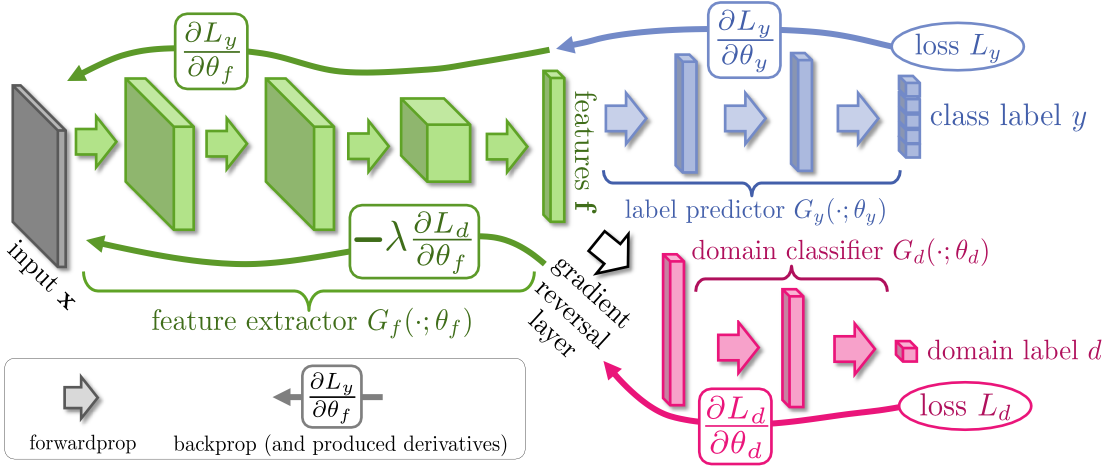
\includegraphics[width=\textwidth]{fig/arch.png}
\caption{Architecture des réseaux adversiaux}
\label{fig:arch}
\end{figure*}

\begin{table*}
\centering
\begin{tabular}{c|c|c|c}
a  & a & a&a\\
\end{tabular}
\end{table*}


Il reste maintenant à déterminer les hyper-paramètres de notre réseau : 
$\lambda_{adapt}$ et l'architecture du réseau.

Puisque l'on ne dispose pas des labels pour les exemples issus du domaine Cible
Il faut trouver un autre moyen pour estimer les performances du modèle.

Ce problème a été abordé dans \cite{Zhong}. La solution proposée (validation 
inversée croisée) consiste à dire que :

Si le modèle $\eta$ est performant sur le domaine Cible alors les labels $D_T^Y$ 
prédis sur les données Cible sont justes. Il est alors possible de s'en servir
pour construire un modèle qui s'adapte dans l'autre sens (du domaine Cible 
vers le domaine Source) et prédire avec précision les labels du domaine Source
que l'on connaît. C'est donc les résultats de ce modèle 'renversé' $\eta_r$ qui 
indiqueront les performances des hyper-paramètres choisis. 

Tout comme dans le cas de la validation simple, cette méthode peut être 
exécutée sur des découpages différents de l'ensemble des données Afin 
d'obtenir une estimation plus fine des performances. 
On met de coté une petite partie des données puis on entraîne les deux modèles
($\eta,\eta_r$) sur la grande partie restante. Finalement l'évaluation 
s'effectue sur la partie mise de coté.

% subsection méthode (end)
% section réseaux_adversiaux (end)
\section{Critiques et questions} % (fold)
\label{sec:critiques_et_questions}

Il m'est assez difficile de donner mon point de vue critique sur cet article
puisque je n'en ai pas lu beaucoup. Je ne connais donc pas vraiment les 
standards de qualité. Cependant il fait sans nul doute parti des articles les 
mieux écris que j'ai lu.

Critiques :
\begin{description}
	\item[+] La section de rappel (section 3) est complète et suffisamment 
	détaillée pour qu'un non-expert puisse comprendre le papier sans avoir
	à aller chercher l'information dans les papiers cités.
	\item[++] L'algorithme 1 contient du vrai code. Clair et utilisant des 
	opérations simples, il est possible pour le lecteur d'implémenter un 
	réseau adversial simple sans avoir à télécharger le code des auteurs
	(qui requiert tout de même une lourde installation).
	\item[+] Le conseil de codage pour les librairies existantes. Si les gens
	s'occupant les librairies populaires de réseau de neurone savent comment 
	implémenter efficacement leur algorithme cela permet de	diffuser bien plus
	aisément leur idée parmi leur collègues dans le monde.
	\item[+] Les expériences sont très détaillés. Peu ou pas d'information 
	concernant les hyper-paramètres ou les données sont manquantes.
	\item[-] Lors de l'annonce du plan dans l'introduction les numéros de 
	sections sont absents ce qui ne permet pas de se rendre directement à 
	la partie souhaitée en première lecture
	\item[-] Il faut attendre la page 5 avant d'entrer dans le vif du sujet.
\end{description}

Questions :
\begin{itemize}
	\item Dans la pratique comment sépare-t-on les couches faisant partie des
	descripteurs des couches de la partie classifieur d'un réseau de neurone ?
	(Ce qu'il faut savoir pour placer la couche de renversement du gradient ?)
	\item Pairwise Poisson binomial Test ?
	\item Comment fonctionne le early stopping ?
\end{itemize}


% section critiques_et_questions (end)
\section{MNIST} % (fold)
\label{sec:mnist}
Dans cette dernière partie je vais résumer mes tentatives pour reproduire
les résultats sur MNIST.

Tout d'abord, mon protocole expérimental diffère de celui des auteurs afin 
de gagner du temps :
\begin{enumerate}
	\item Pas de Validation inversée croisée
	\item Les données de MNIST-M sont construites aléatoirement et je n'ai
	pas trouvé de dataset téléchargeable. Je les ai donc reproduis sur ma 
	machine. Mais elles seront nécessairement un peu différentes de celles 
	utilisées dans l'article.
	\item Pas de convolution mais l'algorithme 1 (code python fourni)
\end{enumerate}

J'ai pu obtenir certains résultats concordant avec ceux de l'article comme par
exemple figure \ref{fig:mnist-to-m}. Où le taux d'erreur sur MNIST-M (environ 
78\%) est très proche de celui donné dans le papier.

\begin{figure}[ht]
\centering
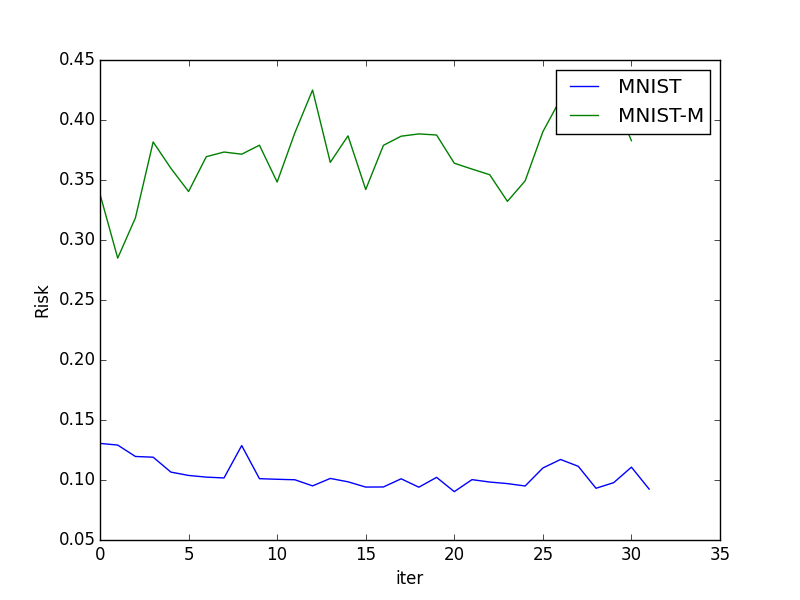
\includegraphics[width=\columnwidth]{fig/mnist-to-m.png}
\caption{Erreur au cours de l'entraînement du DANN de MNIST vers MNIST-M.
($\lambda_{adapt}=0.8$, 50 neurones cachés)}
\label{fig:mnist-to-m}
\end{figure}


Cependant pour un modèle entraîné uniquement sur MNIST sans adaptation, j'ai
obtenu 90\% d'erreur, donc rien de mieux que le hasard contrairement à leur 
expérience qui donnait quand même au alentour de 52\%. Je suppose que 
l'utilisation de réseau à convolution est la principale raison de cette 
différence. En effet les réseaux à convolution vont obtenir des descripteurs
plus adaptés à l'analyse d'image contrairement à une simple couche complètement
connectée.


% section mnist (end)

\bibliography{paper}
\bibliographystyle{icml2016}

\end{document} 


% This document was modified from the file originally made available by
% Pat Langley and Andrea Danyluk for ICML-2K. This version was
% created by Lise Getoor and Tobias Scheffer, it was slightly modified  
% from the 2010 version by Thorsten Joachims & Johannes Fuernkranz, 
% slightly modified from the 2009 version by Kiri Wagstaff and 
% Sam Roweis's 2008 version, which is slightly modified from 
% Prasad Tadepalli's 2007 version which is a lightly 
% changed version of the previous year's version by Andrew Moore, 
% which was in turn edited from those of Kristian Kersting and 
% Codrina Lauth. Alex Smola contributed to the algorithmic style files.  
